\chapter{Overview of CryptDB}
\label{chp:overview_cryptDB}

This chapter provides an overview of CryptDB, starting with the system architecture, followed by its different encryption mechanisms and encryption layer adjustments. Along with the assessment, a small application will be introduced and used as an example to help the reader in understanding the practical and impractical usages of CryptDB.

\section{System Architecture}
\label{sec:sysarc}

CryptDB's architecture is divided into two pieces, a proxy server and a database server as seen in Figure \ref{cryptdb_plain}. The proxy server is an intermediate server placed between the application server (used by the application to manage key set-up and interacting with clients) and the database server. Its purpose is to intercept queries going from the application to the database and anonymize the information of the query, as well as decrypting results going from the database server to the user's application. By doing so, it eliminates the possibility of eavesdropping attackers to obtain any sensible information on the server side.

\begin{figure}[H]
	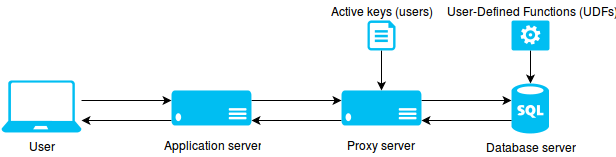
\includegraphics[scale=0.58]{CryptDB_Plain.png}
	\caption{System architecture of CryptDB interacting with a client application.}
	\label{cryptdb_plain}
\end{figure}

Another vital part of the proxy server's domain is to issue queries to the database that adjusts the encryption layer of the columns that the user has issued a query on, which will be discussed in section \ref{adjust_enc_level}. The last responsibility of the proxy server is to keep track of the users that are currently logged in using a table of active keys. In addition to keeping the list of active keys, the proxy server also keeps an embedded database with the schemes of the encrypted tables in the database. By storing this, the proxy server keeps a continuous picture of the encryption layer for each column, which is used for adjusting the encryption layer for a column in order to allow certain types of functionality.

The authors \citep{CryptDB_Main_Paper} have implemented CryptDB both with MySQL and PostgreSQL database management systems. CryptDB requires no modifying of the database system, other than adding a set of \Gls{udf}. \Gls{udf} in CryptDB allows the database to perform cryptographic operations on the encrypted data, as well as adjust the encryption level of different columns.

CryptDB has two operational modes, or principals. One for applications consisting of only one user, and another for multi-user applications. Application keys consists of both a symmetric key rooted in the users application password and a public-key pair. When logging in, the proxy derives encryption keys with the user's password as the root. These keys are used for accessing the data items that are accessible to that particular user and to encrypt new items. When the user logs out, the keys are deleted from the proxy server.



\section{SQL-Aware Encryption and the Onion Scheme}
\label{sec:sqlaware}

\begin{wrapfigure}[17]{r}[1pt]{4cm}
\centering
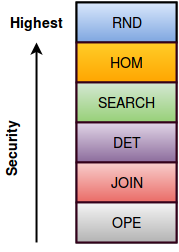
\includegraphics[width=\linewidth]{encstack/enc_stack_ope.png}
\caption{Ordering of the different encryption layers based on the security they provide.}
\label{fig:enc_stack}
\end{wrapfigure}

CryptDB uses an encryption scheme called \emph{SQL-aware encryption} or \textit{onion encryption}. This is a collection of different encryption schemes, each providing different levels of security and computations to be executed. Data items stored using CryptDB are encrypted multiple times using these different schemes, or layers, of encryption. The result is a onion-like structure where the outer layers provide maximum security and low functionality, while the inner layers provide less security, but more functionality. Figure \ref{fig:enc_stack} shows the ordering of the different layers from most secure to least secure. Each layer will be explained throughout this section.

In order to describe the different operations in CryptDB  assume, as a scenario, a simple employee application with a table structure and some example records as shown in Table \ref{demoapp_table}. Our application is created in order to provide some insight in the salary distribution within our firm, with respect to age, number of years within the firm and employment division. EmplNum is the number associated with the employee in other systems and applications, and \gls{ssn} used for creating paychecks for employees and similar operations.

\begin{table}[H]
\centering
\begin{tabular}{| r | r | l | r | r | r | l |}
\hline
  Id & EmplNum & Name & SSN & Age & Salary & Division \\
  int & int & varchar(255) & varchar(255) & int & int & varchar(255) \\
 \hline \hline
 1 & 42 & Alice & 24127312345 & 42 & 440000 & Marketing \\
 2 & 1 & Bob & 17054623456 & 69 & 850000 & Management \\
 3 & 1337 & Charlie & 31129134567 & 23 & 390000 & Engineering \\
 4 & 123 & Donna & 11117945678 & 36 & 510000 & Management \\
 \hline

\end{tabular}
\caption{Employee table for a simple employee application with example records.}
\label{demoapp_table}
\end{table}



\subsection{Random}

\Gls{random_onion} is the highest security level in CryptDB and provides the maximum security found in the encryption scheme. It uses a strong block cipher such as Blowfish or \Gls{aes} in \Gls{cbc_mode} mode and a random \gls{iv} to ensure that the block cipher is probabilistic \citep{CryptDB_Main_Paper}. \Gls{random_onion}, being the maximum security level provided, does not allow any computation to be done on the encrypted data. In other terms, this level is a natural choice for sensitive data that is only meant to be read. When encrypting the same message $m_1$ multiple times with a block cipher that is probabilistic, the resulting ciphertexts $c_1$, $...$, $c_n$ are unequal. 

For example, given two encryptions of the same plaintext $m_1$; $c_1 = Enc_{sk}(m_1)$ and $c_2 = Enc_{sk}(m_1)$ under the same secret key $sk$, the resulting ciphertexts are $c_1$ and $c_2$ such that $c_1 \neq c_2$. \gls{sql} operations supported by this scheme are \verb!SELECT!, \verb!UPDATE!, \verb!DELETE! and \verb!INSERT!. It also supports altering an existing table by removing or adding columns using the \verb!ALTER! statement. In our sample application, the \gls{ssn} would be the most natural thing to stay encrypted under \gls{random_onion} at all times, as there are not many natural operation to perform on such numbers. However, the other columns are not likely to be encrypted under \gls{random_onion} as it is likely that the application would want to perform some operations which demands a lower encryption level. As for an example, take the perhaps most natural query at this encryption level, the \verb!INSERT! statement

\begin{verbatim}
INSERT INTO employee_table
VALUES('', 5, 'Eric', '29026056789', 55, 680000, 'Engineering');
\end{verbatim}

\noindent
which adds a record in the employee table containing Eric's information. When it comes to \verb!SELECT!, \verb!DELETE! and \verb!UPDATE!, it only supports regular queries without the \verb!WHERE! clauses and similar statements:

\begin{verbatim}
SELECT * FROM employee_table;
UPDATE employee_table SET salary = 0;
DELETE FROM employee_table;
\end{verbatim}



\subsection{Homomorphic Encryption}

Another vital part of \Gls{sql} is the ability to perform addition and multiplication. For CryptDB to be able to perform these operations, it utilizes a \Gls{hom_onion} scheme. As previously described, homomorphic encryption is a technique that enables computation on encrypted data without decrypting it first. CryptDB uses Pailler multiplication for enabling additive operations such as \verb!SUM! and \verb!AVERAGE! \cite{Paillier}. If our application is in need of finding out the total sum of the salaries within the firm, we would do something like this

\begin{verbatim}
SELECT SUM(Salary)
FROM employee_table;
\end{verbatim}

\noindent
Multiplication was not initially implemented, but has been implemented in some versions of CryptDB by an outside team using the El Gamal cryptosystem \cite{cryptdb_guidelines}. 



\subsection{Search}

In order to perform a search for words in the encrypted texts, CryptDB has a scheme called SEARCH. This was an implementation of the cryptographic protocol suggested by Song et al. making it almost as secure as the \gls{random_onion} scheme \citep{CryptDB_Main_Paper}. The main idea is to split a text encrypted with SEARCH into individual keywords on a given delimiter specified by the application developer. To enhance the security, duplicate keywords are removed before they are randomly permuted. When executing a search, the server would be given an encrypted token of the keyword, and would retrieve encrypted values matching the token. Originally, SEARCH could perform \texttt{LIKE} operations as other database systems. In the most recent version of CryptDB's software it has been deprecated, as the developers did not have the time to integrate it into the latest version.


\subsection{Deterministic}
\label{sec:det}

As \Gls{random_onion} allows no computation to be done on the encrypted data and \gls{hom_onion} only allows addition, the next layer brings some more functionality to the toolbox. \Gls{deterministic_onion} is an encryption scheme enabling the application to perform standard \gls{sql} operations such as equality checks, distinct, group by and count. By allowing these sorts of computations, the application leaks information to an adversary. In particular, it leaks which ciphertexts that decrypts to the same plaintext value. Following the previous example; if the scheme encrypted the message $m_1$ two times, the resulting ciphertexts $c_1$ and $c_2$ are such that $c_1 = c_2$. For our sample application, \Gls{deterministic_onion} would be the scheme used when allowing operations such as \verb!GROUP BY!, \verb!DISTINCT! and \verb!COUNT!. Continuing with our sample application, we now want to find out what types of departments that exists in our table:

\begin{verbatim}
SELECT DISTINCT Division
FROM employee_table;
\end{verbatim}
\noindent
which returns \verb!Engineering!, \verb!Marketing! and \verb!Management!. As described, a deterministic scheme encrypts the same plaintext to the same ciphertext every time. By taking advantage of this, CryptDB is capable of iterating over the encrypted data and returning a distinct selection of the different ciphertexts observed. At the \gls{deterministic_onion} layer the \verb!WHERE! clause is also supported when running equality checks. An example usage is the query below, where the name, age and salary of all employees from the management division are returned:

\begin{verbatim}
SELECT Name, Age, Salary
FROM employee_table
WHERE Division = 'Management';
\end{verbatim}

\noindent
We could also extract the total salary for each division by using the \verb!GROUP BY! clause along with the \verb!SUM! operation introduced previously:

\begin{verbatim}
SELECT Division, SUM(Salary)
FROM employee_table
GROUP BY Division;
\end{verbatim}

\noindent
For the encryption, \gls{deterministic_onion} uses a strong block ciphers, and either with 64-bit or 128-bit block size. If a value is larger than 128-bits, it leaks  prefix equality when used with \gls{aes} \citep{CryptDB_Main_Paper}.



\subsection{Order-Preserving Encoding}
\label{sec:ope}

Since \Gls{sql} also allows the user to compute on order relations between items, CryptDB introduces an \Gls{ope_onion} scheme \citep{CryptDB_Main_Paper}. This scheme is based on a requirement where the sort order of the ciphertext matches the sort-order of the corresponding decrypted plaintexts. It also requires that the scheme reveals no other information about the plaintexts, other than the respective order. For example, if a value $x \ge y$ then the corresponding encryption would be such that $Enc(x) \ge Enc(y)$. In \Gls{sql}, such an operation is used for order comparison, which are range checks, ranking, sorting, and extracting minimum and maximum values. 

CryptDB uses a modified version of the scheme proposed by Boldyreva et. al \citep{ope_cryptdb} as their \gls{ope_onion} scheme, which is a random order-preserving injective function. An injective function is a one-to-one random mapping function that preserves the order of the elements. Since queries related to order consists of retrieving items between two values, or ranges related to one particular value, the encrypted values can be stored as binary trees at the server, ensuring logarithmic run-time \cite{ope_cryptdb}.


\begin{figure}[h]
	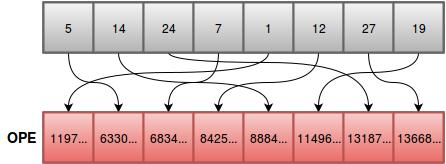
\includegraphics[scale=0.7]{one-to-one.png}
	\caption{Order-preserving encryption of a set of integer values.}
	\label{fig:ope_function}
\end{figure}

Figure \ref{fig:ope_function} shows the order-preserving encryption of a set of integers, where no information is leaked, except for the order of the ciphertexts. When searching for persons in our imaginary firm that has a yearly salary over 500 000, the query uses the \verb!WHERE! clause and then performs an order check where it navigates down the binary three for items that has a salary larger than the requested value.

\begin{verbatim}
SELECT Name, Salary
FROM employee_table
WHERE Salary > 500000;
\end{verbatim}

Popa et al. have also proposed their own \gls{ope_onion} scheme to go with CryptDB \cite{CryptDB_OPE_Encoding} which the claim to be an enhancement of the scheme proposed by Boldyreva, but due to other priorities, this scheme was never actually implemented into CryptDB's software.



\subsection{Equality Join and Order-Preserving Join}

A good database system should be able to join columns. A join is to combine information in two (or more) tables into one by joining the tables on some shared column. CryptDB supports two cases. The first is the regular \gls{eqjoin} between two columns, and the other is \gls{opejoin} which involves order relation checks. Ideally, the proxy server should know in advance which columns that should be allowed to be joined in order to encrypt these column with the same key. Because of the key-chaining approach where each data item is encrypted with a new key, CryptDB is in need of a separate encryption scheme in order to compute joins in a safe manner.

Popa et al. introduce a new cryptographic primitive for equality joins, \gls{join_adj}, which is a deterministic function \citep{CryptDB_Main_Paper}. The idea is to let the proxy server adjust the encryption keys of columns in real-time, based on the observed query. By using this approach, CryptDB protects against the administrator to learn any relations between tables and columns by trying to perform joins on his own. When a join query is observed at the proxy, it sends an adjusted key to the database server enabling it to adjust the values in one of the two affected columns. When an adjustment has been done, the columns share the key until the proxy server issues a new adjustment key to either one of the columns.

The second case is the order-preserving join, which depends on the \gls{ope_onion} scheme previously described. The binary tree structure of the scheme makes in infeasible to use the same approach as \gls{eqjoin}. Therefore, CryptDB has a requirement that columns where such joins are applicable have to be declared by the application beforehand and encrypted under the same key. If this measure has not been addressed, CryptDB will simply encrypt all columns with the same key.

\begin{table}[H]
\centering
\begin{tabular}{| r | r | l | r | l | r |}
\hline
  Id & EmplNum & University & Graduated & Degree & AdjustedGPA* \\
  int & int & varchar(255) & int & varchar(255) & int \\
 \hline \hline
 1 & 42 & HiST & 1993 & B.Sc. & 319 \\
 2 & 1 & NTNU & 1971 & M.Sc. & 305 \\
 3 & 1337 & UiO & 2015 & M.Sc. & 287 \\
 4 & 123 & NHH & 2009 & MBA & 392 \\
 \hline
\end{tabular}
\caption{Educational table for the employee application. \emph{*Because of no support for floating values, the GPA is multiplied by 100 and rounded down.}}
\label{tab:demoapp_education}
\end{table}

Assume that along with the table of employees, there is also a table holding the employees educational information as seen in Table \ref{tab:demoapp_education}. By performing a join between our two tables on the shared employee number EmplNum, it is possible to extract information from the two combined tables as seen below.

\begin{verbatim}
SELECT Name, Division, University, Graduated
FROM employee_table t1
JOIN employee_education t2
ON t1.EmplNum = t2.EmplNum;
\end{verbatim}

\subsection{Wrapping the Layers}

These different layers are wrapped into four different classes or \emph{onions}, namely \texttt{EQ} (Equality checks), \texttt{ORD} (Order relations), \texttt{SEARCH} (Searching) and \texttt{ADD} (Addition) as shown in Figure \ref{cryptdb_onions}. Each onion has a special purpose in means of supporting certain operations, and every data item is encrypted each of the different onions using the different layers. However, the application does not necessary maintain all of the onions. There is, for example, no need for maintaining the ADD-onion if the data item is a string type.

\begin{figure}[H]
	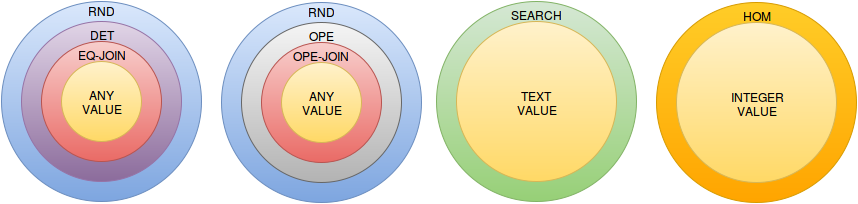
\includegraphics[scale=0.42]{Onions.png}
	\caption{Overview of the structure of the SQL-aware encryption scheme. From left: The EQ-onion, ORD-onion, SEARCH-onion and ADD-onion.}
	\label{cryptdb_onions}
\end{figure}


\section{Adjusting the Encryption Level Based on the Query}
\label{adjust_enc_level}

We have seen that there is an encapsulation of different encryptions for each data item, and our ideal scenario is that our data is encrypted at the highest, feasible level at all times.  But how is the system supposed to perform a range check if the utmost layer is the \gls{random_onion} which does not support any functionality at all?

CryptDB solves this particular case gracefully by having the proxy server observe incoming queries in real-time. As previously mentioned, the CryptDB proxy server has an embedded table that stores the current encryption layer of all columns. After observing a query, it checks this table whether or not the current encryption level of the inflicted columns are supporting the query. For example in our sample application, the user has issued the query:
\begin{verbatim}
SELECT *
	FROM employee_table
	WHERE salary > 5000000;
\end{verbatim}

Keep in mind that all data items at this point are encrypted with \gls{random_onion} as the utmost layer. What the proxy does, is that before sending the rewritten query to the database server, it sends an \verb!UPDATE! query first. This query orders the database server to remove the outer encryption level of the ORD-onion to match the \gls{ope_onion} layer, before it sends the rewritten query. Figure \ref{ope_layer_adjustment} illustrates how the proxy server observes the query, and issues the \verb!UPDATE! query. \verb!SET! is used to change the current encryption level of the ORD-onion, and \verb!cryptdb_decrypt_int_sem! is the name of the UDF that the server will use to adjust the encryption layer to  support the query. The curious string \verb!'???]???G??+?,?#'! is the encrypted key which the server will use along with the UDF.

\begin{figure}[h]
	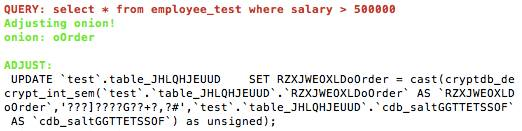
\includegraphics[scale=0.7]{terminal/adjustOnionLayer.jpg}
	\caption{Encryption layer adjustment performed by proxy server upon receiving a query.}
	\label{ope_layer_adjustment}
\end{figure}

After performing the encryption layer adjustment, the proxy rewrites the query as shown in Figure \ref{rewritten_query}. As described, each of the columns are anonymized upon the creation of a table. The proxy server keeps table schemes with a mapping between the encrypted column in the database server, and the actual decrypted name of the column. By doing so, it is able to substitute the different parts of the query so it matches the encrypted columns in the database. For the record, 'test' is the name of the current database.  

\begin{figure}[h]
	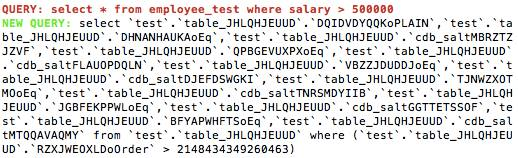
\includegraphics[scale=0.7]{terminal/executeQuery.jpg}
	\caption{Rewritten query to be sent to server after encryption level adjustment.}
	\label{rewritten_query}
\end{figure}

When a layer has been stripped off, it does not automatically get re-encrypted unless the developer has specified such actions. For example, if an irregular query forces the encryption level lower than necessary. For applications running in single-mode, the encryption layers will over time be in a stable state supporting the relevant queries. But, for multi-mode applications, the developer decides the functionality, hence the types of queries that the application can produce. Therefore, it is possible to start application at the correct layers based on the desired functionality, and the proxy does not perform any encryption level adjustments at all.



\section{Security}

In section \ref{sec:sysarc}, two different modes for using CryptDB were mentioned. For applications built for one particular user, the single-user mode of CryptDB is used. Examples of applications where such a mode would be useful is when creating a personal diary application or a contact list application. When building applications consisting of multiple users with their own usernames and passwords, the developer needs to use the multi-user mode.

\subsection{Single-user Mode}
If an application is created with a single user in mind, then it should be running in the single-user mode where the encryption keys are derived from one secret master key rooted in the application's password (the password to the database). By running in this particular mode, the user has access to all data encrypted through the proxy server. In this mode, both the proxy server and the application server are considered to be trusted. The database server, however, is considered to be untrusted and subject to the snooping of a curious database administrator owning the server system that is hosting the database. As of the most recent versions of the CryptDB software, only the single-user mode is supported, which has been used to create a small demo application presented in Chapter \ref{chp:software}.

\subsection{Multi-user Mode}
Picture a simple online discussion forum, where users can interact by posting messages to discussion boards or sending each other private messages. As described in Section \ref{chp:database_Security}, database applications are in need of access control in order to restrict access to certain tables based on the user's credentials, hence the need for declaring user entities as well as different groups. But how can a user read messages on the discussion board if they are encrypted by another user's key? What about private messages, which suffer from the same case, as they will be encrypted with the sender's key? CryptDB solves these cases by letting developers use annotations in their schemas.


Annotations are in most languages and frameworks used for describing code and attributes, as well as inducing different behaviours, and are usually parsed at compile time. In CryptDB, the annotations is used when creating database schemas, and then used by the software to perform different types on encryptions based on the annotated attributes. Table \ref{annotations} shows a basic use of such annotations. \verb!PRINCTYPE! is used to annotate external users, which are authenticated through the access control by providing their password, and internal users, which are entities inside the database. \verb!ENC_FOR! is used to indicate which columns that contain sensitive data, and in the next column CryptDB needs to store which principals that should have access to the sensitive column. We see that we have access to the column, but how can we decrypt something encrypted with someone else's keys?

\begin{table}[h]
\begin{Verbatim}[frame=single]
\textcolor{red}{PRINCTYPE} physical_user \textcolor{red}{EXTERNAL};
\textcolor{red}{PRINCTYPE} user, msg;

CREATE TABLE privmsgs (
	msgid integer,
	subject varchar(255)	\textcolor{red}{ENC_FOR} (msgid msg),
	msgtext text		\textcolor{red}{ENC_FOR} (msgid msg) );

CREATE TABLE privmsgs_to (
	msgid integer,
	recvid integer,
	sendid integer,
	(sendid user) \textcolor{red}{SPEAKS_FOR} (msgid msg),
	(recvid user) \textcolor{red}{SPEAKS_FOR} (msgid msg) ); 
\end{Verbatim}
\caption{Use of policy annotations in database schemas when creating multi-user applications. Annotations are highlighted in red.}
\label{annotations}
\end{table}

CryptDB chains encryption keys used to encrypt columns or data items to the root key, which is the user's password. The \verb!SPEAKS_FOR! annotation gives a principal access to all the keys that the principal it speaks for has access to. For example in Table \ref{annotations}, both the user sending the private message and the user receiving it, speaks for the principal type \verb!msg! and thereby has access to all the keys of the \verb!msg! entity. This means that the secret key of the message is encrypted two times, first with the sender's key and then with the receiver's key.

Consider this case: Alice wants to send a private message to Bob, which means that the private message needs to be encrypted two times using both Alice and Bob's secret keys. Keys of users who are logged in are kept in a table at the proxy server, but what happens when the proxy server needs to encrypt something with a key which at the time is inaccessible? The keys that are used by a principal to encrypt data consists of both a symmetric key and an asymmetric key pair. When both parties are logged in, the proxy uses their symmetric keys to encrypt the message. If Bob is currently logged out, the message is encrypted using his public key so that he can decrypt it using his corresponding private key when he logs in.

As previously mentioned, the current version of CryptDB has only the option of developing single-mode applications. One may react to the fact that the developers has stopped maintaining such a useful way of developing applications with multiple user's and interaction between users. However, Mylar \cite{mylar_homepage} is the creators of CryptDB's new project. Mylar addresses the threat of the insecure proxy server being compromised by an attacker, and how to protect the confidentiality of the users' data in such events. In the event of an attack on the proxy server in CryptDB, the only parties that are compromised are those who are currently logged in, as their keys are stored at the proxy server and accessible to the attacker.


\subsection{Securing Applications When Using CryptDB}
\label{sec:sensitive}

Another importance related to the use of annotations is the \verb!SENSITIVE! annotation. By labelling columns as \emph{sensitive}, CryptDB provides strong security guarantees of the data stored in the affected columns and also semantic security \cite{popa_thesis}. When a column is marked as sensitive, the only encryption schemes that are allowed are \gls{random_onion}, \gls{hom_onion}, SEARCH and, if the column has the \verb!UNIQUE! constraint from \gls{sql}, \gls{deterministic_onion}. The reason for enabling the \gls{deterministic_onion} scheme under a constraint of the data being unique, is as there are no equal plaintexts, there will be no equal ciphertexts, and the scheme leaks no information about the encrypted data.



\section{Functional Limitations}
\label{sec:limits}

\gls{fhe} is nowhere near being practical yet, but CryptDB tries its best to be a somewhat practical \gls{he} scheme allowing a set of operations that they claim to be enough to support 99.5\% of all queries observed in an \gls{sql} trace from a production MySQL server \citep{CryptDB_Main_Paper}. However, there are multiple fairly trivial data types that CryptDB does not support.

For example, all fixed-point types and floating-point types are not supported, meaning that computing on decimal values are difficult for the application to perform. In Table \ref{tab:demoapp_education}, our GPA-column, where the most natural data type would be decimal, has been adjusted to an integer by the application. One way to cope with the limitations is to let the developer be responsible for transforming a data type that is not supported into a supported one, and handle the inverse transformation upon receiving an encrypted result. Another option is to let CryptDB exclusively store such values as text with \gls{random_onion} or \gls{deterministic_onion} encryption, and let the client perform operations on such data types. Obviously neither options are desirable, as it is quite the opposite of the goal when using schemes such as CryptDB. 

Floating points are not the only unsupported data types. Data types related to date and time, namely Timestamp, Date, Time, DateTime, Year and NewDate are neither supported, giving us a bit of a headache. In other terms, if your application needs to encrypt dates and at the same time be able to compute on them, you are in bad luck. The authors suggestion is to encrypt each part of a date (day, month, year, second, minute, hour and so on) in separate columns, and perform the computations on those columns instead of a composite date column.

Could we possibly used Unix timestamps, which are integers representing the number of seconds since 1st of Januar 1970 (given that the application does not need any dates before the startpoint of Unix time)? By representing dates as integer values, we lose a lot of functionality, as we are only able to compute the order of the dates. As soon as we want to retrieve dates within a specific year, we need to retrieve all data items and perform the operation on the client side, or do a range query for dates between two values. When performing the range query, we need to compute the upper and lower Unix timestamps of our interval. The downside with this approach is that it forces the encryption layer down to \gls{ope_onion}, which is the most insecure encryption scheme in CryptDB. By storing the different parts of the date in separate columns, we are able to keep the encryption layer to \gls{deterministic_onion} for most date related queries. 

While the three-column approach is rather complicated, it works surprisingly well for our demo application. Assume that we add some more columns to Table \ref{demoapp_table} with the precise date of birth in stead of age as seen in Table \ref{tab:empl_date}.

\begin{table}[H]
\centering
\begin{tabular}{| c | r | r | r | c |}
\hline
  ... & Day & Month & Year & ... \\
  ... & int & int & int & ... \\
 \hline \hline
 ... & 24 & 12 & 1973  & ... \\
 ... & 17 & 05 & 1946 & ... \\
 ... & 31 & 12 & 1991 & ... \\
 ... & 11 & 11 & 1979  & ... \\
 \hline

\end{tabular}
\caption{Additional columns to the employee table with date properties stored in separate columns.}
\label{tab:empl_date}
\end{table}

Consider 17th of May 1980 as our test date, and that we want all employees born after this point in time. In a regular database system supporting date related data types, our query would be something like this on a concatenated date of birth column

\begin{verbatim}
SELECT Name, date_of_birth
FROM employee_table
WHERE date_of_birth > '17/5/1980'
ORDER BY date_of_birth ASC;
\end{verbatim}

As for CryptDB, where such queries do not return anything meaningful, we need to modify our approach as seen below

\begin{verbatim}
SELECT Name, Day, Month, Year
FROM employee_table
WHERE (year = 1980 and month = 5 and day > 17)
OR (year = 1980 and month > 5)
OR (year > 1980)
ORDER BY year ASC, month ASC, day ASC;
\end{verbatim}

Queries are also subject to some constraints. In \gls{sql}, users are also allowed to use \emph{subqueries} or \emph{nested queries}, which is an \gls{sql} query embedded inside another using the \verb!WHERE! clause to bind them together. Such subqueries are used by the main query to retrieve data that will be used as a condition in order to further restrict its result. If we now want to retrieve salaries for employees' graduating after 1980, a regular \gls{sql} query would be something like this

\begin{verbatim}
SELECT Name, Salary
FROM employee_table
WHERE EmplNum IN
    (SELECT EmplNum
    FROM employee_education
    WHERE graduated > 1980);
\end{verbatim}

In CryptDB, such queries are infeasible, which leaves us with two options. Option one is to perform a join instead of using subqueries. While this may solve our problem in this particular situation, it does not necessary work in all situations and may create duplicated rows in the result. Option two is to let the application execute the operation as two separate queries and store the result of the first query as an intermediate value used in the second query.

\begin{verbatim}
temp_result :=
    SELECT EmplNum
    FROM employee_education
    WHERE graduated > 1980;

SELECT Name, Salary
FROM employee_table 
WHERE EmplNum IN (temp_result);
\end{verbatim}


Along with complicating tables and adding overhead to the database, such limitations also puts the responsibility of the developer to add software code on the application server or client side. For larger applications and complex operations, such actions are not necessarily feasible and hence an limitation on the use of CryptDB as a database system.\\